\section{Introdução e Motivação}

\begin{frame}{Roteiro}
  \begin{columns}
    \begin{column}{0.5\textwidth}
      \begin{itemize}
        \item \textbf{Parte 1: Caso de Estudo}
        \begin{itemize}
          \item Alocação de Água no DF
          \item Trabalhos de Referência
          \item A Instância Hídrica
        \end{itemize}
        \vspace{0.3cm}
        \item \textbf{Parte 2: Formulação e Algoritmo}
        \begin{itemize}
          \item Fluxo de Custo Mínimo (MCF)
          \item Grafo Residual e Otimalidade
          \item Algoritmo SSP e Complexidade
        \end{itemize}
      \end{itemize}
    \end{column}
    \begin{column}{0.5\textwidth}
      \begin{itemize}
        \item \textbf{Parte 3: Demonstração e Resultados}
        \begin{itemize}
          \item Execução Iterativa SSP
          \item Resultados da Alocação
          \item Limitações e Sensibilidade
        \end{itemize}
        \vspace{0.3cm}
        \item \textbf{Parte 4: Conexão Estocástica}
        \begin{itemize}
          \item Pontes de Schrödinger
          \item O Poder da Incerteza
          \item Conclusão
        \end{itemize}
      \end{itemize}
    \end{column}
  \end{columns}
\end{frame}

\subsection{O Problema de Alocação de Água}
\begin{frame}[shrink=5]{O Problema de Alocação de Água}
  \begin{block}{Contexto Real}
    Como distribuir água potável de forma eficiente a partir de Estações de Tratamento de Água (ETAs) para as Regiões Administrativas (RAs) do Distrito Federal?
  \end{block}
  
  \begin{itemize}
    \item \textbf{Desafio}: Equilibrar a capacidade instalada de produção (supply) e as demandas locais das RAs (demand).
    \item \textbf{Custos}: Perdas físicas, infraestrutura e, principalmente, custo de bombeamento (energia elétrica).
    \item \textbf{Pergunta Central}:
  \end{itemize}

  \begin{exampleblock}{Pergunta}
    Dado o grafo de adutoras, qual é a alocação de fluxo que atende a todas as demandas minimizando o custo total de transporte?
  \end{exampleblock}
\end{frame}

\subsection{Trabalhos de Referência}
\begin{frame}{Trabalhos de Referência}
  Nossa modelagem é inspirada em estudos de transporte ótimo em redes hídricas:
  
  \begin{itemize}
    \setlength{\itemsep}{15pt}
    \item \textbf{Mascherpa et al. (2023)}:
      Uso de transporte ótimo regularizado para modelar o fluxo de água e contaminantes em redes de distribuição.
    \item \textbf{Mascherpa et al. (2026)}:
      Estimação de contaminação sob incerteza e observabilidade da rede.
  \end{itemize}
\end{frame}

\begin{frame}{Abordagem Determinística e Escopo}
  \small
  \begin{itemize}
    \setlength{\itemsep}{8pt}
    \item \textbf{Modelo Determinístico (SSP)}: Foco no algoritmo \textit{Successive Shortest Path} para resolver o fluxo de custo mínimo sem incertezas na demanda.
    \item \textbf{Implementação do Zero}: Desenvolvimento puro do resolvedor, sem depender de pacotes ou solvers externos prontos.
    \item \textbf{Complexidade Estocástica}: A inserção de incertezas nas demandas tornaria o problema estocástico e altamente complexo (frequentemente NP-difícil).
    \item \textbf{Fundamentação Básica}: A modelagem determinística é etapa inicial obrigatória antes de qualquer extensão estocástica.
  \end{itemize}
\end{frame}

\subsection{Do Modelo à Aplicação Real}
\begin{frame}{Do Modelo à Aplicação: O Caso de Estudo}
  Para validar o resolvedor desenvolvido, aplicamos a modelagem a um cenário real e crítico:
  
  \begin{block}{Caso de Estudo: Alocação Hídrica no Distrito Federal}
    A infraestrutura de distribuição de água potável da CAESB pode ser descrita como uma rede de fluxo, onde:
    \begin{itemize}
      \item \textbf{Estações de Tratamento (ETAs)} agem como fontes de suprimento de água.
      \item \textbf{Regiões Administrativas (RAs)} agem como sumidouros (demandas locais).
      \item \textbf{Adutoras} representam arcos de tráfego com custos de bombeamento específicos.
    \end{itemize}
  \end{block}
\end{frame}

\subsection{A Instância Simplificada}
\begin{frame}{A Instância Hídrica do Distrito Federal}
  \begin{itemize}
    \item \textbf{Topologia}: Grafo bipartido com 7 ETAs (fontes) e 7 RAs (sumidouros), interconectados por 26 adutoras.
    \item \textbf{Dados}: Baseados em estatísticas reais da CAESB e ADASA.
  \end{itemize}
  
  \begin{table}
    \centering
    \tiny
    \begin{tabular}{llr}
      \toprule
      \textbf{Nó} & \textbf{Tipo} & \textbf{Balanço Nodal (l/s)} \\
      \midrule
      ETA Rio Descoberto & Fonte & $+4450.00$ \\
      ETA Brasília & Fonte & $+1200.00$ \\
      ETA Lago Norte & Fonte & $+700.00$ \\
      ETA Sobradinho & Fonte & $+570.00$ \\
      ETA Gama & Fonte & $+320.00$ \\
      ETA Paranoá & Fonte & $+300.00$ \\
      ETA Planaltina & Fonte & $+60.00$ \\
      \midrule
      Plano Piloto & Sumidouro & $-1763.40$ \\
      Sobradinho & Sumidouro & $-1101.09$ \\
      Guará & Sumidouro & $-1067.97$ \\
      Taguatinga & Sumidouro & $-1051.42$ \\
      Planaltina & Sumidouro & $-927.23$ \\
      Samambaia & Sumidouro & $-852.72$ \\
      Ceilândia & Sumidouro & $-836.17$ \\
      \bottomrule
    \end{tabular}
  \end{table}
\end{frame}

\begin{frame}{Topologia da Rede Hídrica do DF}
  \centering
  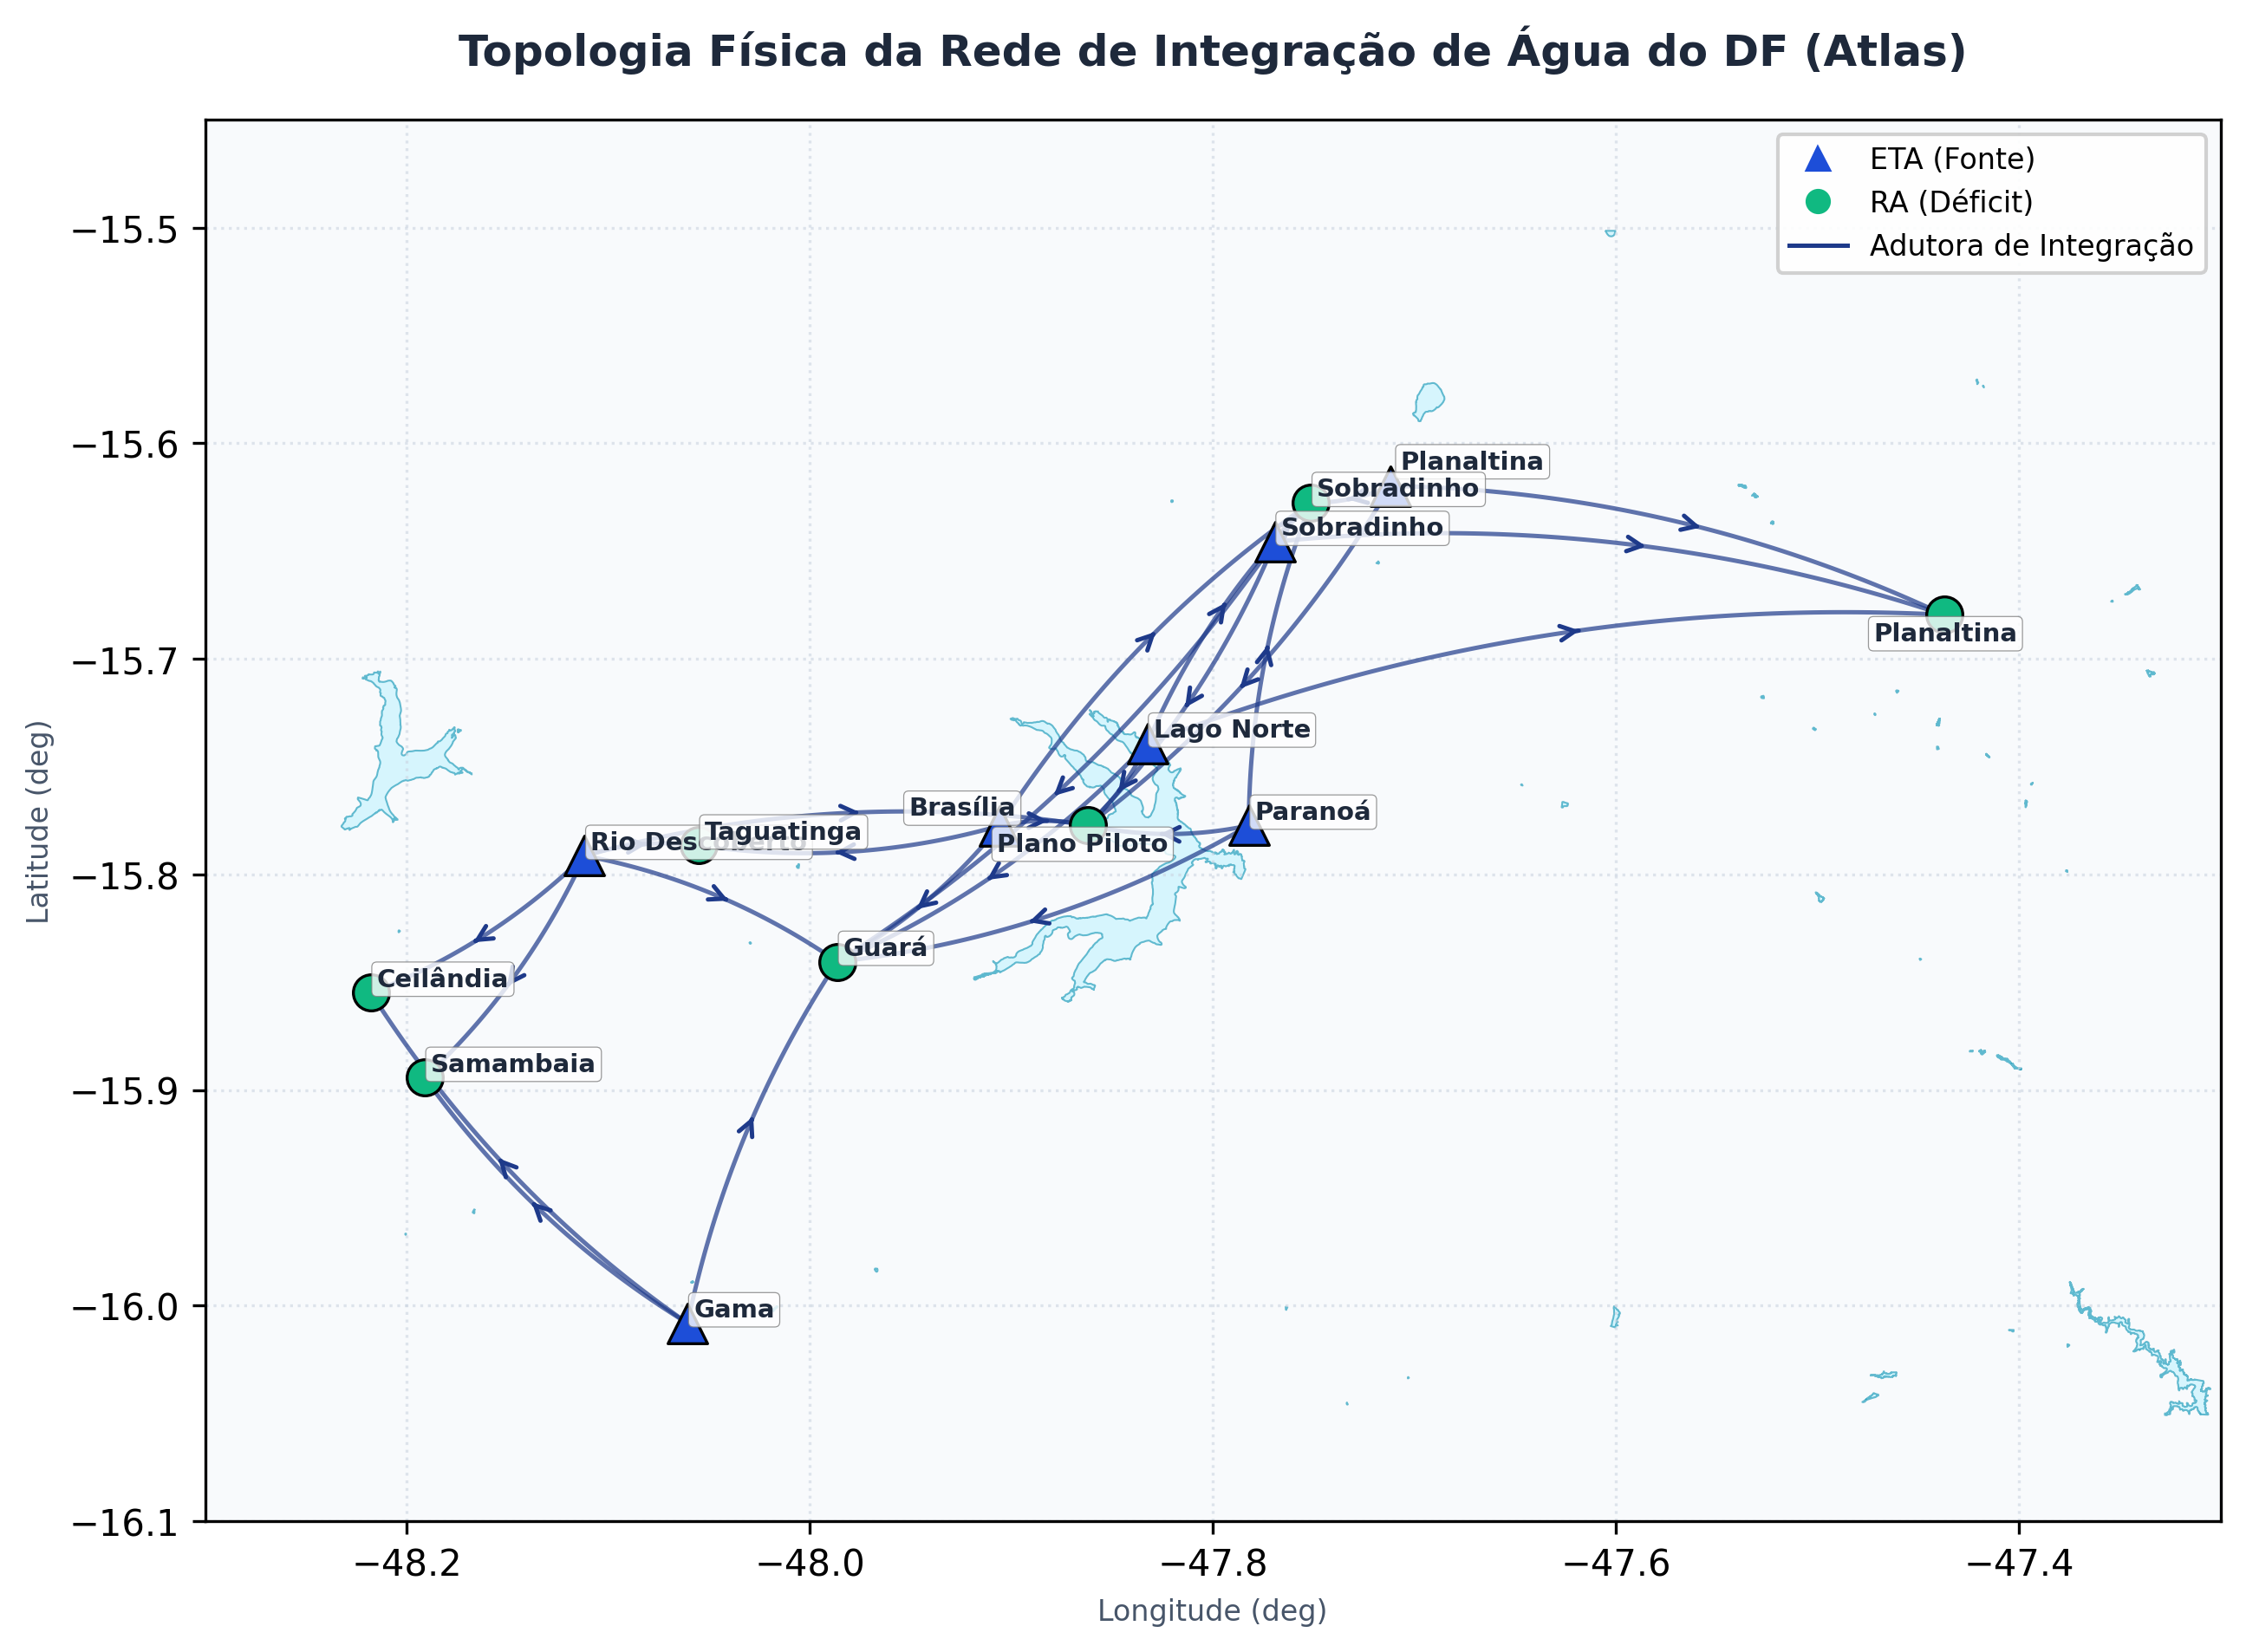
\includegraphics[width=0.85\textwidth]{figuras/mapa_topologia.png}
  
  \scriptsize Rede Hídrica Base (Capacidade e Distância)
\end{frame}

\subsection{O Que Queremos Como Saída}
\begin{frame}[shrink=10]{O Que Queremos Como Saída}
  \begin{itemize}
    \item \textbf{Objetivo}: Encontrar o plano de fluxos ótimos $x_{ij}^*$ para cada adutora.
    \item \textbf{Visualização dos Fluxos}: Arestas mais espessas representam fluxos maiores, enquanto arestas ociosas tornam-se inativas.
  \end{itemize}
  \centering
  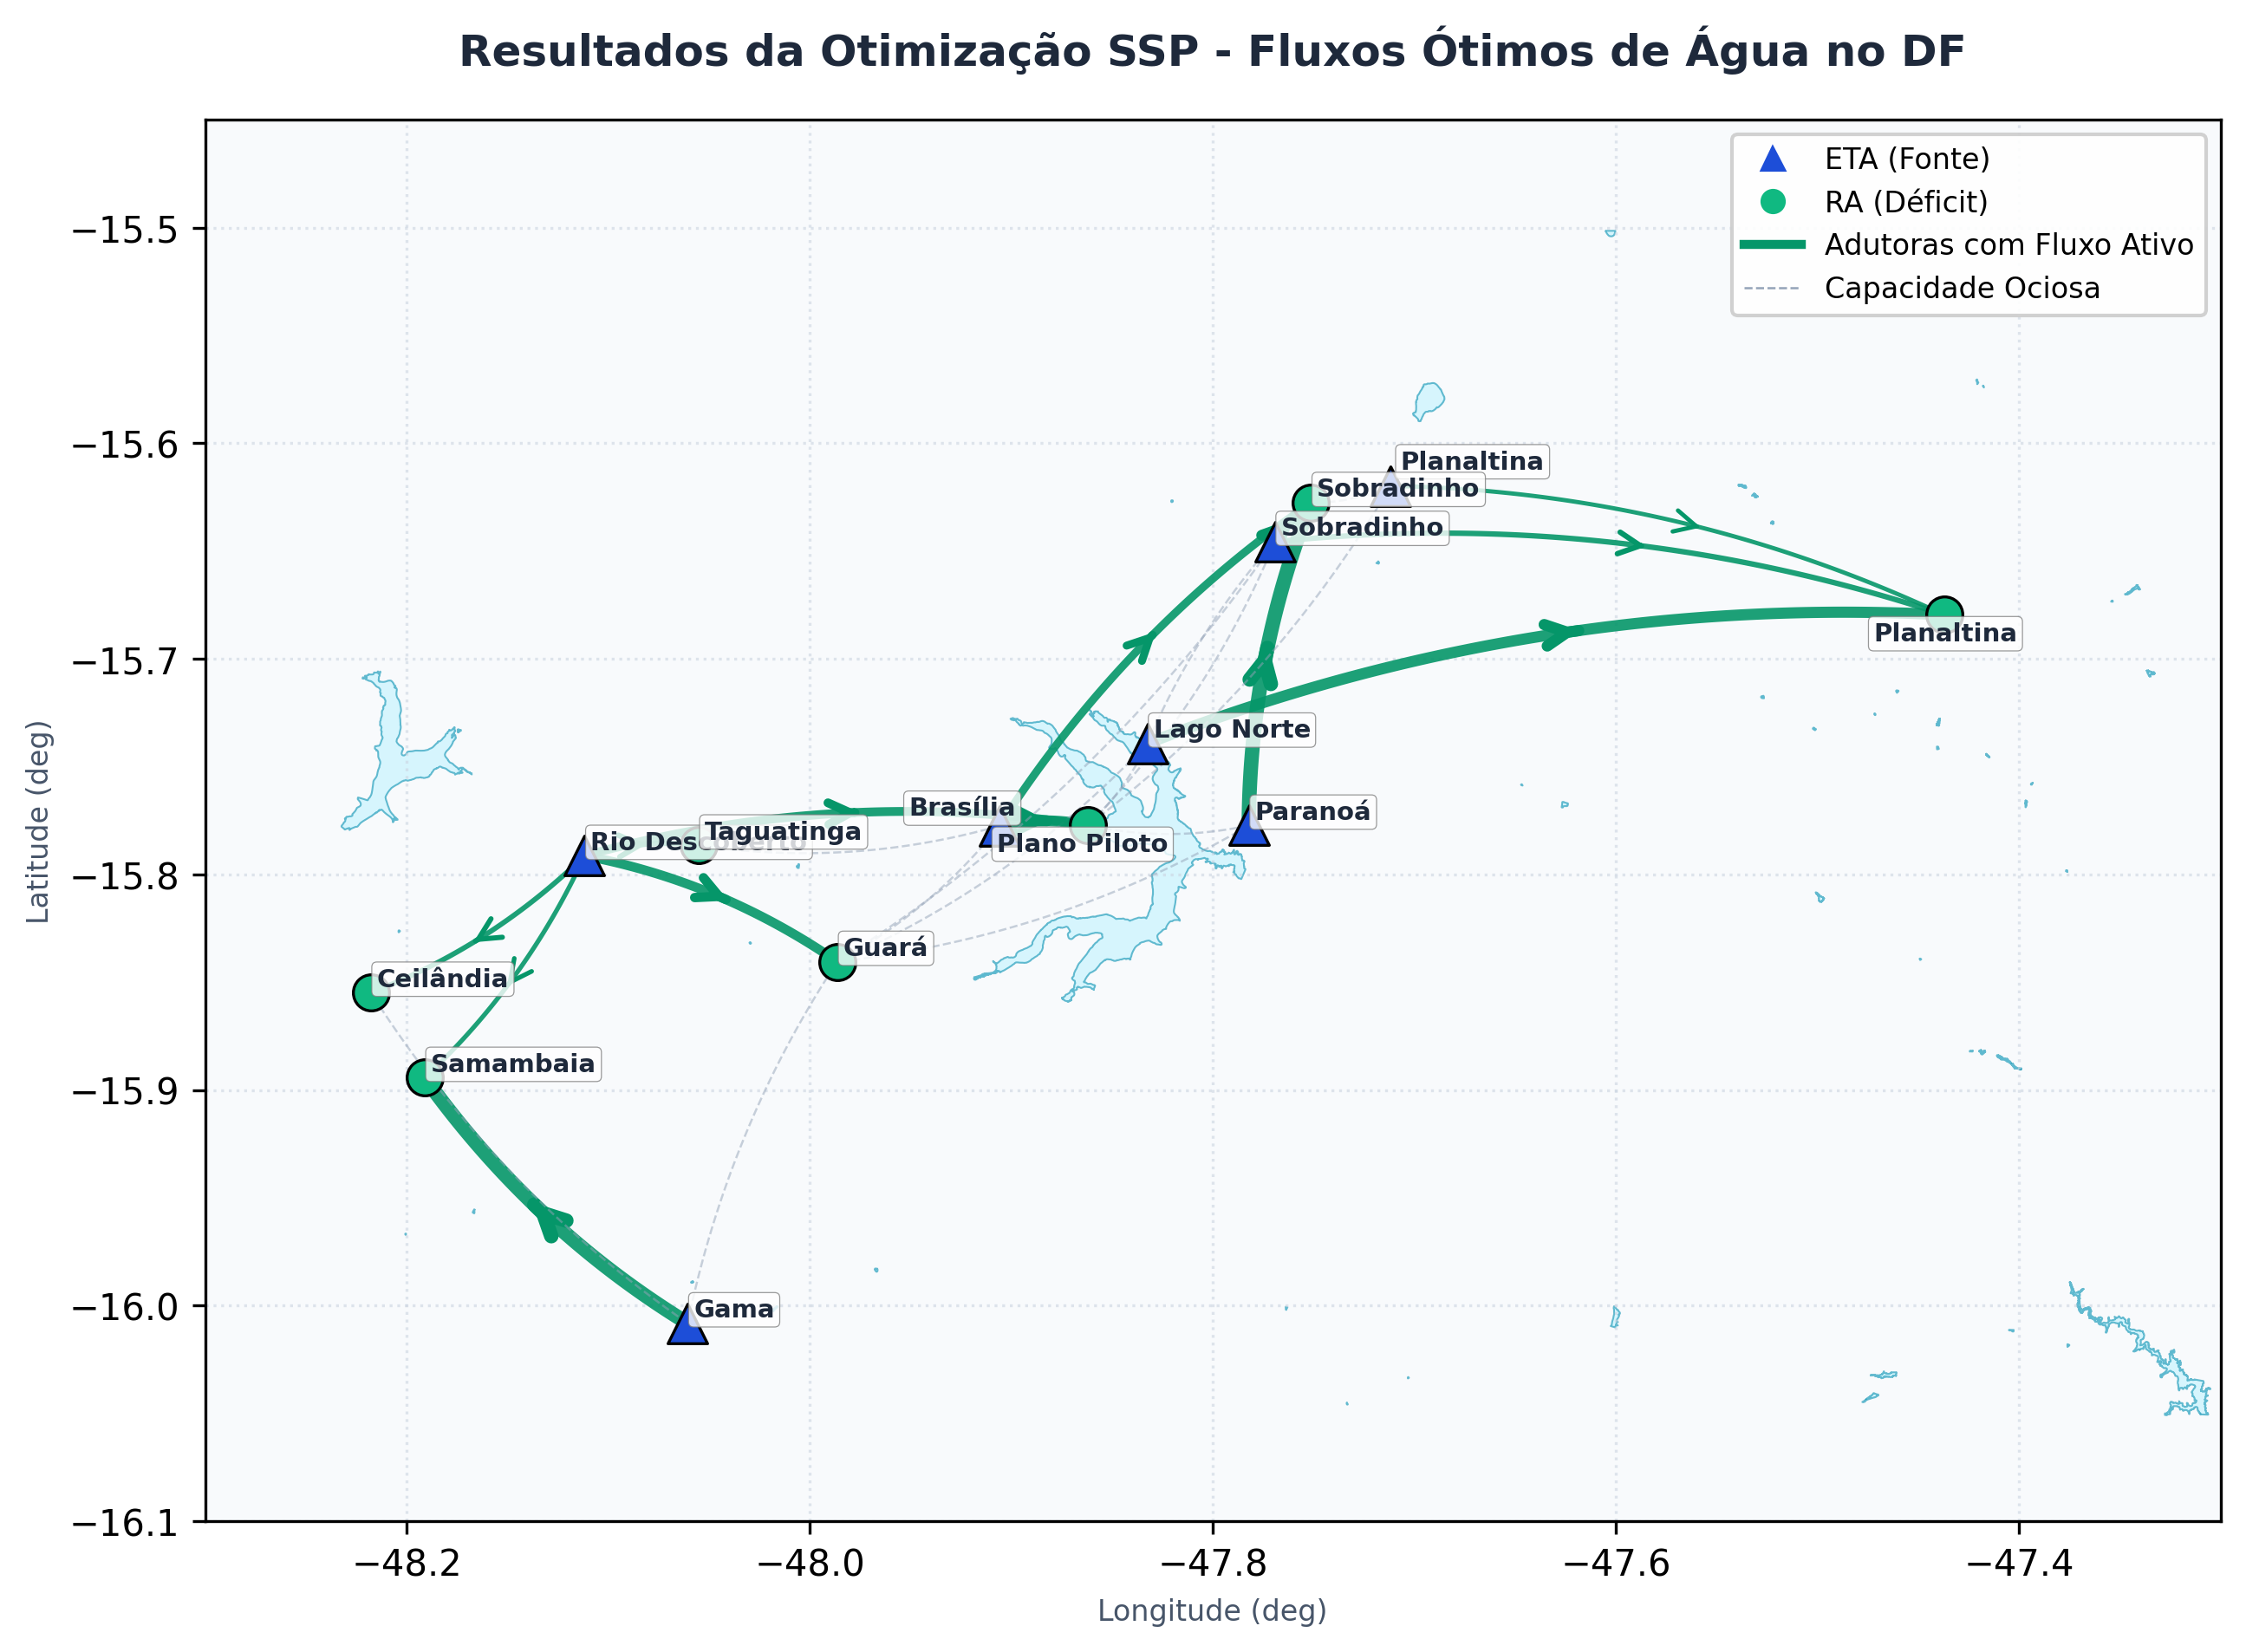
\includegraphics[width=0.45\textwidth]{figuras/mapa_fluxos_otimos.png}
  
  \scriptsize Visualização Prévia do Fluxo Ótimo SSP
\end{frame}